\documentclass[12pt]{article}
\usepackage{graphicx, amsmath}
\graphicspath{ {./} }
\setlength{\oddsidemargin}{0.25 in}
\setlength{\evensidemargin}{-0.25 in}
\setlength{\topmargin}{-0.6 in}
\setlength{\textwidth}{6.5 in}
\setlength{\textheight}{8.5 in}
\setlength{\headsep}{0.75 in}
\setlength{\parindent}{0 in}
\setlength{\parskip}{0.1 in}

\begin{document}
\thispagestyle{plain}
   \newpage
   \setcounter{page}{1}
   \noindent
   \begin{center}
   \framebox{
      \vbox{\vspace{2mm}
    \hbox to 6.28in { {\bf BioE 131: Intro to Computational Biology}
                        \hfill Fall 2020 }
       \vspace{4mm}
       \hbox to 6.28in { {\bf \Large \hfill Probability  \hfill} }
       \vspace{2mm}
       \hbox to 6.28in { {\it Professor: Ian Holmes \hfill} }
      \vspace{2mm}}
   }
   \end{center}
   {Notes written by Vikram Shivakumar}
   \vspace*{4mm}


\section{Introduction}
\textbf{Random processes} are present in all branches of biology, from population genetics and ecology to molecular simulations and systems biology. How can we study processes that are inherently random (or seem to be random)? We can build probabilistic models, and describe random systems using \textbf{probability theory}. In this note, we will cover basic definitions of core probability theory concepts (like random variables, distributions, Bayes' Theorem), as well as some probabilistic models used in biology.

\section{Probability Theory}
\subsection{Basic Definitions}
A \textbf{random variable} is a variable that has multiple possible values, each with an associated probability. Given a random variable (often abbreviated \textit{RV}) $x$, which can take on a set of values $X$, we can define the probability of a value $a \in X$ to be $P(x = a)$, which is often just written as $P(x)$ as a shorthand.\\[10pt]
A \textbf{probability distribution} is the probability of each possible value an RV can take. There are two types of distributions, \textbf{discrete}, with a finite set or countably infinite (i.e. integers) set of values, and \textbf{continuous}, with an (uncountable) infinite set of values, like all real numbers. In both scenarios, the probability of all possible values must add up to 1 (the normalization constraint):
$$\sum\limits_{x\in X}P(x) = 1\text{ (where }P(x)\text{ is a \textbf{probability distribution})}$$
$$\int\limits_{x=0}^{\infty}p(x)dx = 1\text{ (where }p(x)\text{ is a \textbf{probability density function} or \textbf{pdf})}$$
Along with a PDF, continuous functions also have a cumulative density function (CDF), which describes the probability of an outcome less than a given value:
$$P(x\leq a) = \int\limits_{-\inf}^ap(x)dx
$$
\subsection{Conditional, Joint, and Marginal}
A \textbf{joint probability}, $P(x, y)$ between two variables $x$ and $y$, defines the distribution over the combinations of possible values for both RVs. The \textbf{marginal distribution} can be found by "summing out" an RV from the joint distribution, taking the sum over all possible values of the RV:
$$P(x) = \sum_yP(x,y)$$
$$P(y) = \sum_xP(x,y)$$
The \textbf{conditional probability}, $P(x|y)$, is the probability of an event $x$ given that $y$ has occurred:
$$P(x|y) = \frac{P(x,y)}{P(y)}$$
The normalization constraints still hold for conditional and joint distributions:
$$\sum_x\sum_yP(x,y) = 1$$
$$\sum_xP(x|y) = \frac{\sum_xP(x,y)}{P(y)} = 1\text{  }\forall y$$
Joint distributions can also be continious, and the above formulas hold (just replace the sums with integrals).
\subsection{Independence}
Two random variables are independent if the distribution of one variable remains the same given an outcome from the other variable, or as an equation:
$$P(x|y) = P(x) \text{ if }x,y\text{ independent}$$
If two RVs are independent, then the joint probability $P(x,y)$ is just the product $P(x)P(y)$.\\[10pt]
As a biological example, pick any two random positions from a genome. The nucleotide for each position is assumed to be independent, because, for example, the probability of selecting an "A" at one position does not change depending on what base is at the other position. However, selecting \textit{adjacent} nucleotides in a genome is not independent, since some pairs of nucleotides are more common than others.\\[10pt]
If two random variables are independent and have the same probability distribution, we call them \textbf{IIDs}, or independent and identically distributed random variables. An example of a sequence of IIDs is rolling $N$ dice, or even rolling the same die $N$ times. This is also an example of a \textbf{uniform} IID, where the probability of any outcome is the same (the probability distribution is flat).
\subsection{Expectation}
The \textbf{expectation} of a distribution, or the expected value $E[x]$, is the sum of all the possible outcomes, weighted by their probabilites:
$$E[x] = \sum_{x\in X}xP(x)$$
The variance of the distribution can be found with the equation:
$$V[x] = \langle x^2\rangle-(\langle x\rangle)^2$$

\subsection{Probability Distributions}
An example of a discrete distribution is the \textbf{Binomial distribution}, which models the probability of $k$ successes out of $n$ trials, where the probability of a success is $p$. The distribution can be described by:
$$f(k;n,p) = P(K=k) = \binom{n}{k}p^k(1-p)^{n-k}$$
where
$$\binom{n}{k} = \frac{n!}{k!(n-k)!}$$\\
The \textbf{Gaussian} or \textbf{Normal distribution} is an example of a continuous distribution, with a PDF of the general form:
$$P(x) = \frac{1}{{\sigma \sqrt {2\pi } }}e^{{{ - \left( {x - \mu } \right)^2 } \mathord{\left/ {\vphantom {{ - \left( {x - \mu } \right)^2 } {2\sigma ^2 }}} \right. \kern-\nulldelimiterspace} {2\sigma ^2 }}}$$
where $\mu$ is the mean (or center of the distribution), and $\sigma$ is the standard deviation.\\[10pt]
Another example of a continuous distribution is the \textbf{Extreme Value (Gumbel) Distribution} or \textbf{EVD}. This distribution models the probability of the max (or min) value of $N$ RVs of another distribution. For example, when aligning two random proteins, many alignments are possible, but we are interested in the \textit{best} alignment. Thus the EVD describes the distribution of the \textit{best} alignments between two random proteins.\\[10pt]
We can extend this example by looking at a protein homology search. For each protein in the database, we can take the best alignment score with our query, and create a distribution of the best alignment scores across the database. We can then model this distribution of alignments scores as an EVD, and calculate the probability (or $p$ value) of a given score using the CDF of the distribution.

\subsection{Bayes' Theorem}
\textbf{Bayes' theorem} is used widely in statistical inference, and describes the probability of an event given prior knowledge:
$$P(x|y) = \frac{P(y ,x)}{P(y)} = \frac{P(y |x)P(x)}{P(y)}$$
A common interpretation is that $x$ is the model that describes $y$, the data. Thus we calculate the \textbf{likelihood} of the data given a model, $P(y|x)$, and weight the likelihood by the \textbf{prior probability} $P(x)$. This is normalized by the evidence probability $P(y)$ to yield the \textbf{posterior probability}, $P(x|y)$, which is the probability of the model given all the evidence.

\subsection{EM and K-means}
Given a set of points, one common task is to cluster the points into groups. From a statistical viewpoint, we can assume that each cluster of points is from a distinct distribution, which are added up to form the full set of points, or the \textbf{mixture model}.\\[10pt]
We can then build a model $\theta$ which represents the different clusters and assign each point $y_i$ to a cluster $x_i$. The likelihood of the model is then given by $P(x,y|\theta)$, which we can weight by the prior probability $P(\theta)$ (if we have no prior knowledge of the models, we can just use a \textbf{uniform prior}). Thus clustering the set of points involves just calculating $$
\text{argmax}_{x,\theta} P(x,\theta|y)$$ which finds the model and assignments which maximize the posterior probability.\\[10pt]
One very common algorithm for clustering is the K-means algorithm, which involves assigning $N$ points to $k$ clusters:
\begin{enumerate}
    \item Start by randomly assigning all the points to $k$ clusters
    \item Find the centroid of each cluster
    \item Assign each point to the nearest centroid
    \item repeat steps 2-3 until the assignments converge
\end{enumerate}
The K-means algorithm is a type of \textbf{Expectation Maximization} or \textbf{EM} algorithm. EM algorithms involves alternating between an expectation (assigning points to the nearest centroid), and maximization (calculating the centroids) steps, run until convergence. The algorithm is used to fit models of the form $P(x,y|\theta)$, where $x$ and $y$ are the hidden and observed data, and $\theta$ represents the model parameters we are trying to fit.

\section{Random Processes in Biology}
Now we will discuss a few random processes and probabilitic models used in various biological problems.
\subsection{Markov Process}
\subsubsection{Formulation}
A Markov process describes a stochastic sequence of states, where the probability of encountering a state only depends on the previous state (called the \textbf{Markov Property}). As an equation:
$$P(x_{n+1} |x_{n},x_{n-1}, x_{n-2},\ldots) = P(x_{n+1} |x_{n})$$
In other words, given the present state, the probability of the future and past states are independent.\\[10pt] 
If there are $N$ states, we can then define the probability of transitioning from state $i$ to state $j$ as $Q_{ij}$, where $Q$ is the \textbf{transition matrix}. We also define the probability of being in state $j$ at timestep $n+1$ as $p_j^{[n+1]}$, which can be calculated by summing over the previous possible states at timestep $n$:
$$p_j^{[n+1]} = \sum_ip_i^{[n]}Q_{ij}$$
\begin{figure}[ht!]
    \centering
    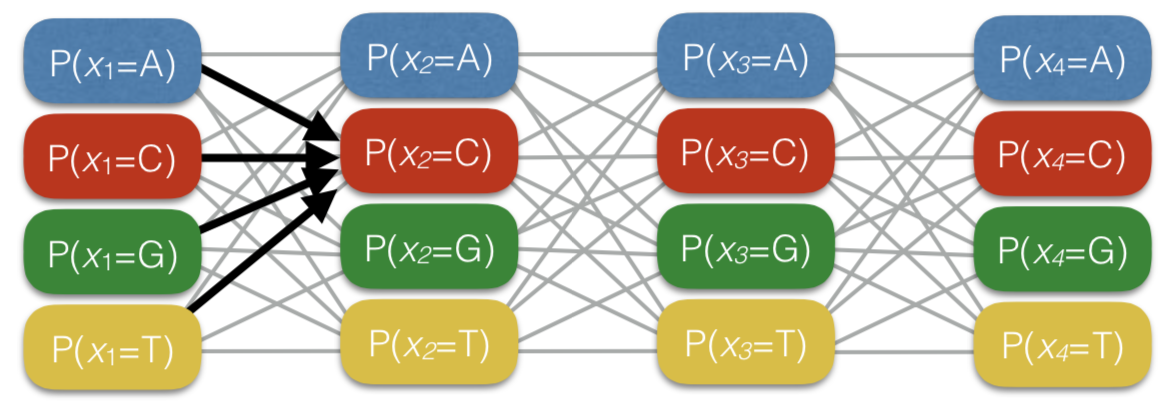
\includegraphics[width = .7\linewidth]{markov_base.png}
    \caption{Markov Chain of a 4nt DNA sequence}
    \label{fig:markov}
\end{figure}
\subsubsection{Examples}
One example of a Markov process is a \textbf{random walk}, a simulation of a Markov process over integers. Each state in the Markov chain is an integer, connected to the previous and next integer with some probability. By simulating multiple timesteps of the Markov chain, we can create a random walk along the chain.\\[10pt]
One example of this is the \textbf{Birth-Death process}.
\begin{figure}[h]
    \centering
    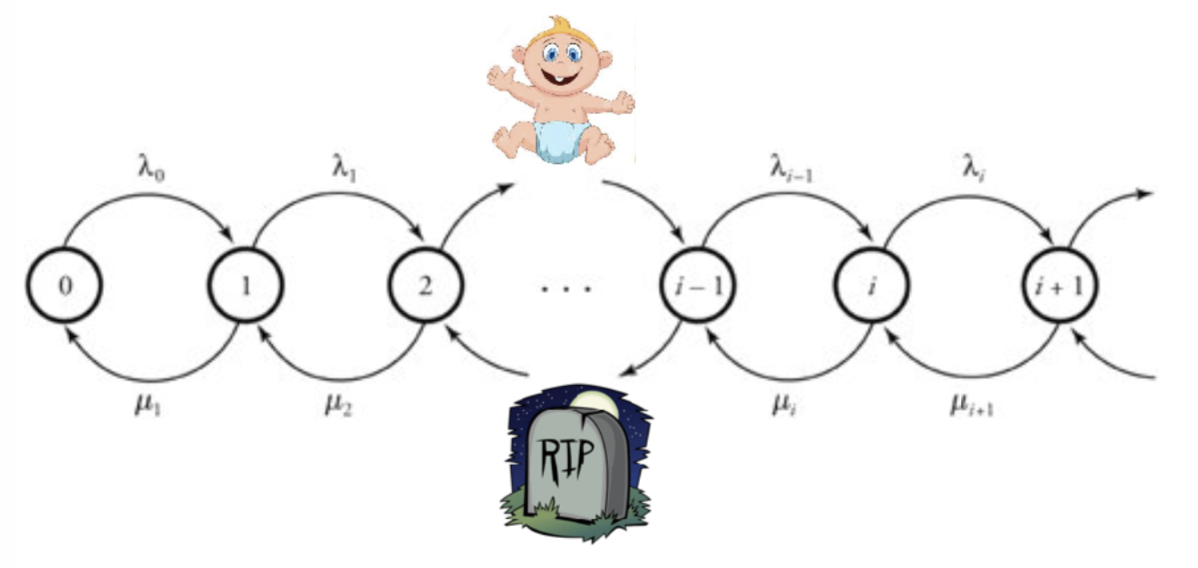
\includegraphics[width = .7\linewidth]{bd_proc.png}
    \caption{Diagram of a birth-death process}
    \label{fig:bd}
\end{figure}
This Markov process over the set of integers is parametrized by two rates: the birth rate ($\lambda_n$) and the death rate ($\mu_n$). At each timestep $n$, the two rates dictate the probability of a birth and death, moving between states which represnt the current population size. We can also add in the concept of immigration, which increases the population like a birth.\\[10pt]
Birth-death processes are used in the \textbf{Unified Neutral theory of Biodiversity}, a model developed by Hubbell (2001) that describes speices diversity in ecological communities. This model uses nested birth-death processes to describe seperate mainland (slow timescale) and island (fast timescale) populations, with immigration between them, to accurately predict species distributions in ecological systems.\\[10pt]
The concept of a birth-death process is also used in the \textbf{tkf91 model}. This model describes sequence evolution, including indels (insertions and deletions of bases), which is similar to the idea of immigration in a birth-death process.
\subsubsection{Hidden Markov Models}
Hidden Markov Models (or HMMs), are a type of Markov model, where each state also emits an observable value. HMMs can describe processes where there is an underlying hidden state, but we can only observe a sequence of \textbf{emissions}, which we can use to reconstruct the hidden states. One example of this is classifying GC-rich regions in a DNA sequence. The probability of outputting a G or C in a GC-rich region is different than in AT-rich regions, but given a DNA sequence we can't tell which positions are in GC or AT-rich regions. These region assignments are the hidden states, while the DNA sequence is the sequence of observable states.\\[10pt]
HMMs are represented by a graphical model, also called a \textbf{Bayes net} or \textbf{factor graph}.
\begin{figure}
    \centering
    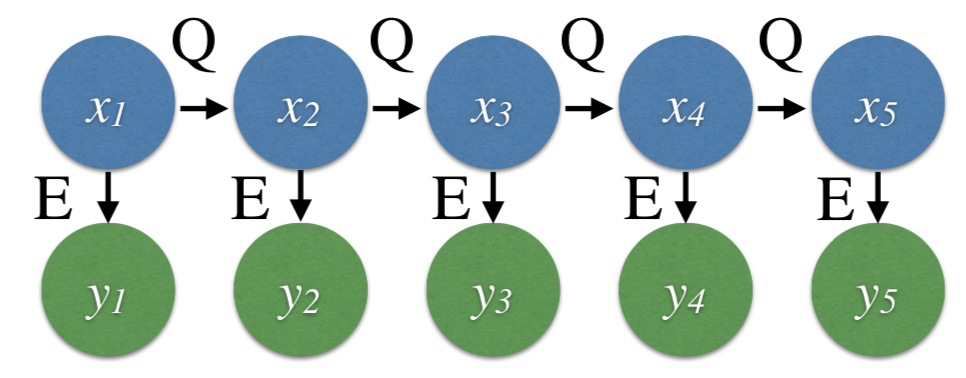
\includegraphics[width = .7\linewidth]{hmm.png}
    \caption{An example hidden markov model (hmm)}
    \label{fig:hmm}
\end{figure}
Bayesian networks describe the conditional relationships between multiple random variables using a directed graph.

\subsection{Hardy-Weinberg equilibrium}
The Hardy-Weinberg principle states that under ideal conditions, the frequency of alleles in a population will remain constant in equilibrium. For example, for a gene with two alleles (A, a), $P(A) = p$, and $P(a) = q$, after a single generation, we get the following genotype frequencies:
$$P(AA) = p^2, P(Aa) = 2pq, P(aa) = q^2$$
Since $p$ and $q$ must sum up to 1, we get:
$$P(A) = P(AA) + \frac{P(Aa)}{2} = p(p+q) = p$$
This principle holds under certain conditions:
\begin{enumerate}
    \item The genome is \textbf{diploid}
    \item There is an \textbf{infinite population}
    \item Mating is random (\textbf{no selection})
    \item The gene locus is \textbf{biallelic}
\end{enumerate}
\subsection{Wright-Fisher model}
The Wright-Fisher model describes the number of alleles in a population over time. Given a gene with 2 alleles (A, a): in generation $t$, assume there are $X_t$ copies of allele A in the population of size $N$. The Wright-Fisher model describes the number of copies of A in generation $t+1$ to follow a binomial distribution:
$$p_{ij} = P(X_{t+1} = j | X_t = i) = \binom{2N}{j} \left( \frac{i}{2N} \right) ^j\left(1-\frac{i}{2N}\right)^{2N-j}$$
where $i$ is the number of copies of allele A in generation $t$ and $j$ is the number of copies in generation $t+1$. One important property of the model is the \textbf{fixation probability}, where the probability of allele A fixing in the population (becoming the only allele, or $2N$ copies in the population), or disappearing altogether, is:
$$P(X_t \text{ absorbs at }2N) = \frac{X_0}{2N}$$
$$P(X_t \text{ absorbs at }0) = 1-\frac{X_0}{2N}$$
where $X_0$ is the initial number of copies of allele A. 
\subsection{Coalescent process}
The Wright-Fisher model can be used to analyze how populations change through time. But what if we want to model how a current population developed? We can essentially run Wright-Fisher \textit{backwards in time}! This is the idea behind the \textbf{Coalescent process}, which can be used to model the probability of two individuals in a population sharing a common ancestor.
\section{Summary}
Random processes appear frequently in biological problems, and one method for modelling them in computational biology is with probabilistic models. Using these models, we can make statistical inferences, characterize the behavior of stochastic processes, and analyze randomness in biological systems.
\end{document}

%topics not covered:
%equilibrium distributions, time-reversibility,detailed balanced in markov chains, all the examples for bayes theorem, crispr guide probabilities



